\documentclass[journal, onecolumn]{IEEEtran}
\usepackage[utf8]{inputenc}
\usepackage{cite}
\usepackage{amsmath,amssymb,amsfonts}
\usepackage{algorithmic}
\usepackage{graphicx}
\usepackage{textcomp}
\usepackage{xcolor}
% 支持中文的宏包，请使用 XeLaTeX 或 LuaLaTeX 编译
\usepackage{xeCJK} 

\begin{document}

\title{驾车者是否在通话？使用蜂窝信号进行移动设备定位}

\author{Shichen Zhang, Student Member, IEEE, Huacheng Zeng, Senior Member, IEEE, \\ Y. Thomas Hou, Fellow, IEEE}

\maketitle

\begin{abstract}
开车使用手机是导致驾驶员分心的主要原因，并引发了大量的交通事故。虽然监控摄像头可用于检测违规使用手机的行为，但在某些场景下（如黑暗和遮挡）效果不佳，并且可能引发隐私担忧。在本文中，我们提出了 PhoLoc，这是一种路侧设备，利用手机发射的蜂窝信号来检测私家车内违规使用手机的行为。PhoLoc 配备了两个传感器：一个多天线无线电接收机和一个低成本激光雷达。它联合处理来自这两个传感器的多模态数据，以估计车辆中手机的相对位置。PhoLoc 的核心推动技术是一种新的近场定位方案，该方案能够通过窃听移动手机的蜂窝信号来估计其在特定时刻的位置。我们已经构建了 PhoLoc 的原型，并在现实场景中评估了其性能。实验结果表明，PhoLoc 在检测通话违规行为方面实现了 4.2\% 的误报率（False Positive Rate）和 13.8\% 的漏报率（False Negative Rate）。
\end{abstract}

\begin{IEEEkeywords}
蜂窝网络定位，无线定位，违规使用手机，交通安全
\end{IEEEkeywords}

\section{引言}

根据美国国家公路交通安全管理局（NHTSA）的研究，驾驶员使用手机的普遍现象是 2021 年美国 553,000 起财产损失事故、248,000 人受伤和 3,211 人死亡的主要原因 [1]。许多国家和地区（例如英国、欧洲和中国）已经立法禁止驾驶员在驾驶时使用手机。能够执行法律并警示分心驾驶员的路侧交通基础设施对于提高驾驶安全至关重要。一种自然的方法是在路边部署高分辨率监控摄像头来检测驾驶员违规使用手机的行为 [2]。然而，摄像头监控系统在黑暗、恶劣天气条件或驾驶员故意隐藏手机等场景下可能无法正常工作。更重要的是，公共区域的摄像头监控可能会引发对驾驶员和乘客隐私的严重担忧。

基于摄像头的交通监控系统的局限性和担忧促使研究人员探索检测驾驶员违规使用手机的替代方案。例如，智能手机传感器如全球定位系统（GPS）和惯性测量单元（IMU）已被研究用于以日益复杂的方式检测分心驾驶行为 [3]–[9]。车内射频识别（RFID）传感系统也被开发用于检测驾驶员的分心驾驶行为 [10]–[12]。然而，IMU 和 RFID 传感器只能在车内使用，不能部署在路边以执行安全法规。这就需要一种既能检测违规使用手机，又能在各种天气条件下表现良好并尊重驾驶员隐私的路侧传感器。

在本文中，我们提出了 PhoLoc，这是一种路侧设备，用于检测私家车驾驶员违规使用手机（驾驶时通话）的行为。图 1 展示了 PhoLoc 的基本思路和应用场景。它配备了两个传感器：一个多天线无线电接收机和一个低成本（约 40 美元）激光雷达。无线电接收机窃听手机发射的蜂窝信号，以估计其在给定时刻的位置（例如图 1 中的 $(x_{0},y_{0})$），而激光雷达用于测量车辆距离 $y_{s}$ 和首次检测到车辆前端的时刻 $t_{s}$，这可用于推断车辆长度。PhoLoc 联合处理来自这两个传感器的数据，以估计车辆速度、车辆长度和手机在车内的相对位置（即图 1 中的 $\Delta x$ 和 $\Delta y$），并利用该相对位置来确定电话是否由驾驶员拨打。

% [图片占位]
\begin{figure}[htbp]
\centering
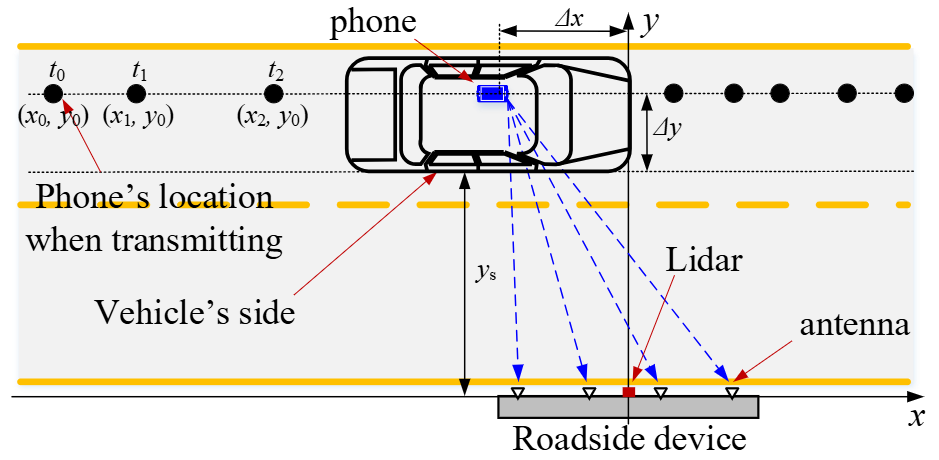
\includegraphics[width=0.8\linewidth]{figures(is_driver)/fig1.png}
\caption{图 1：PhoLoc 示意图。}
\label{fig:1}
\end{figure}

手机定位（估计给定时刻手机的位置）是 PhoLoc 的核心组件。其设计面临三个挑战。
第一个挑战源于车辆的高移动性。对于固定的路侧设备，不同的车辆可能以宽范围的不同速度行驶（例如，从 20 mph 到 45 mph）。此外，PhoLoc 没有车辆速度的先验知识。它必须联合估计车辆速度和手机位置。
第二个挑战源于 VoIP 数据流量的低数据包率，这是 4G LTE 及更高版本蜂窝网络中支持通话的方式。根据 VoIP 协议（G.729 [13]），语音通话期间的 VoIP 数据包率可能低至每秒 25 个数据包。这与我们对真实电话通话的实验观察一致。蜂窝信号的稀疏性使得在给定时刻准确估计手机位置变得困难。
第三个挑战在于车辆是一个富散射环境。毫无疑问，车内手机发射的无线电信号在到达 PhoLoc 天线之前会经过视距（LoS）和非视距（NLoS）路径。由于大多数车辆的框架由金属材料制成，NLoS 路径可能不可忽略。不可忽略的 NLoS 路径的存在使得在高速下准确定位手机具有挑战性。

虽然已经为移动设备开发了许多无线定位技术（例如 [14]–[19]），但大多数技术都是基于 AoA（到达角）或 ToF（飞行时间）的估计来推断信号源的位置。目前尚不清楚，即使可能，这些技术如何在多径丰富的场景中用于定位具有高移动性和流量稀疏性的无线设备。

为了应对上述挑战，我们提出了一种使用线性天线阵列定位移动设备的新方案。我们的设计灵感来自天文干涉仪（特别是新墨西哥州的 VLA [20]）。我们设计的核心思想是增加天线间距（例如 5 英尺），使天线阵列具有大孔径。大天线孔径将远场定位问题转化为近场定位问题，从而可以利用车辆（手机）的移动在给定时刻生成集中的位置模式。具体而言，PhoLoc 将定位问题表述为一个优化问题，并通过最大化测量信道与其在车辆轨迹上的投影 LoS 分量之间的互相关性，来搜索手机在给定时刻的最佳位置值（例如图 1 中的 $(x_{0},y_{0})$）。

所提出的近场定位方案的一个关键问题是信道估计。为了让 PhoLoc（作为窃听者）估计其自身与手机之间的信道，它需要两个设备之间进行细粒度的时间和频率同步，以及手机上行链路参考信号的知识 [21]。此外，蜂窝基站的动态资源分配和用户调度给 PhoLoc 的信道估计增加了另一个挑战。即使可能，估计信道也会给 PhoLoc 带来沉重的计算负担。为了解决这个问题，PhoLoc 利用其天线上的信号相位差来定位目标设备，这可以从原始基带信号中提取，从而消除了信道估计的需要。基于这个想法，PhoLoc 开发了一种低复杂度的手机定位信号处理流水线，既不需要时间/频率同步，也不需要信道估计。由于大多数先前的基于 AoA 和 ToF 的定位技术都依赖于信道状态信息（CSI），这是我们方案与现有方案之间的另一个关键区别。

基于新的定位方案，PhoLoc 通过联合处理来自两个传感器（无线电和激光雷达）的多模态数据来执行系统集成和优化。它利用车辆被检测到的持续时间和私家车的平均长度来估计车辆速度，这可能不准确，但可以显着减少求解所制定的优化问题的时间。此外，PhoLoc 分析从车辆窃听到的蓝牙信号，以确定驾驶员是在进行手持通话还是免提通话。

我们使用带有 5 英尺间隔的四天线 USRP N310 无线电设备和低成本激光雷达传感器构建了 PhoLoc 原型。我们将 PhoLoc 部署在当地道路旁，并以不同的速度（从 10 mph 到 30 mph）驾驶车辆以评估其性能。在我们的实验中，电话是从车辆的不同座位（驾驶员座、副驾驶座、左后座和右后座）拨打的。实验结果表明，PhoLoc 在检测驾驶员通话违规方面实现了 4.2\% 的误报率（FPR）和 13.8\% 的漏报率（FNR）。

本文的贡献总结如下：
\begin{itemize}
    \item PhoLoc 提出了一种近场定位方案，用于估计移动设备在给定时刻的位置。与先前的定位方案不同，所提出的方案不需要用于定位的信道知识。
    \item PhoLoc 结合了两种截然不同的传感器，无线电和激光雷达，以定位车内手机的相对位置。据我们所知，这是第一个在高速下估计移动设备相对位置的工作。
    \item PhoLoc 已在现实场景中进行了评估。实验结果证实了 PhoLoc 在现实应用中的可行性和有效性。
\end{itemize}

\section{预备知识}

美国大多数电话运营商（例如 AT\&T、Verizon 和 T-Mobile）已于 2022 年正式关闭了其 3G 网络 [22]。此后，4G 及更高版本成为提供电话服务的主导蜂窝网络。接下来，我们将描述与 PhoLoc 相关的 4G 网络的关键特征。我们注意到 5G 具有与 4G 相似的信号结构和协议栈。因此，PhoLoc 也适用于 5G 移动设备。

\textbf{上行链路频率和带宽}。不同的电话运营商（例如 AT\&T、Verizon 和 T-Mobile）使用不同的频段为用户提供服务。幸运的是，每个电话运营商的频道信息都是公开的，可在其网站上查阅。在美国，4G 上行链路信道频率主要在 650-900 MHz 和 1700-2100 MHz 范围内 [23]。每个信道的带宽为 20 MHz，采样率为 30.72 MSps。虽然 4G 标准支持 TDD 和 FDD 模式 [24]，但大多数美国蜂窝网络在 FDD 模式下工作。

\textbf{用于通话的 VoIP}。当手机进行语音通话时，它将向其蜂窝塔发射信号（即上行链路传输）。VoIP [25] 用于在 4G 及更高版本的网络中传输语音数据。G.729 和 G.711 是 4G 网络中 VoIP 最常用的两种编解码器。根据 3GPP [26]，移动 VoIP 连接每秒至少发送 25 个 VoIP 数据包；VoIP 数据包大小范围从 60 字节到 280 字节。正如我们的实验所示，通话的数据包间隔可能高达 40 毫秒。VoIP 使用较小的带宽进行射频信号传输。显然，VoIP 的小带宽非常适合 PhoLoc 的位置估计。

\textbf{上行链路信号传输}。在 4G 网络中，每个用户设备（UE）基于基站（BS）周期性广播的主同步信号（PSS）和辅同步信号（SSS）获取小区/扇区 ID 和帧定时。UE 还使用 PSS 和 SSS 将其载波频率与服务基站同步。时间提前量（Timing Advance, TA）由基站用于通知 UE 需要提前多少时间进行上行链路传输。上行链路使用单载波频分多址（SC-FDMA）[27] 调制方案进行信号传输。每个 UE 使用一个或多个资源块（RB，由 12 个子载波和 7 个 OFDM 符号组成）进行数据传输。解调参考信号（DMRS）是基于小区和扇区 ID 生成的，包含在每个 RB 中用于基站的信道估计。鉴于 4G 网络的复杂性，对于窃听者（PhoLoc）来说，估计其自身与手机之间的信道并非易事。

\textbf{上行链路资源分配}。蜂窝网络是一个集中式系统。基站是中央控制器。在上行链路中，时间和频率资源由基站动态分配 [28]。因此，手机发射的信号频率随时间变化。正如稍后将展示的，手机发射的无线电信号在短时间内（约 0.1 毫秒）是窄带的，但在长时间内（约 1 秒）其频率跨度超过 20 MHz。

\section{移动设备的近场定位}

\subsection{问题表述}
考虑一个移动单天线发射机和一个固定的多天线探测器（无线电接收机），如图 2 所示。发射机以恒定速度 $v$ 沿平行于探测器线性天线阵列的方向移动，起始位置为 $(x_{0},y_{0})$。在其移动过程中，发射机在时刻 $t_{i}, i=0,1,2,\dots,N_{s}$ 发送数据包。探测器在时刻 $t_{i}$ 接收数据包并估计其自身与发射机之间的信道。为了便于说明，我们假设发射机具有单天线。通常，我们的方法适用于发射机具有多天线的情况。

% [图片占位]
\begin{figure}[htbp]
\centering
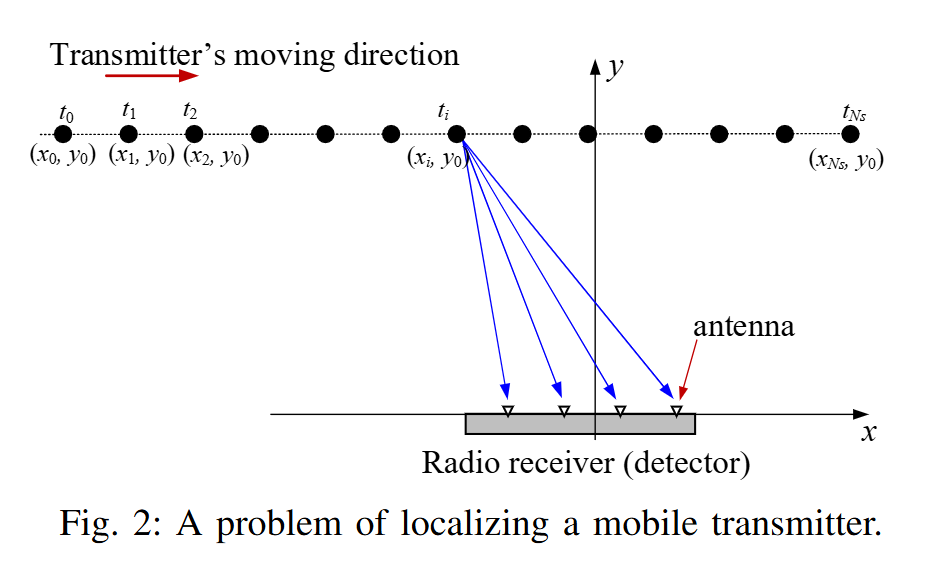
\includegraphics[width=0.8\linewidth]{figures(is_driver)/fig2.png}
\caption{图 2：定位移动发射机的问题。}
\label{fig:2}
\end{figure}

设 $M$ 为探测器的天线数量。设 $\vec{h}_{i}=[h_{1i},h_{2i},...,h_{Mi}]$ 为时刻 $t_{i}$ 的测量信道。那么，我们有
\begin{equation}
h_{mi}=\alpha_{mi0}\cdot e^{-j2\pi\frac{d_{mi0}}{\lambda}}+\sum_{l=1}^{L}\alpha_{mil}\cdot e^{-j2\pi\frac{d_{mil}}{\lambda}},
\end{equation}
其中 $\alpha_{mil}$ 是时刻 $t_{i}$ 发射机到探测器第 $m$ 个天线的第 $l$ 条路径的信号幅度衰减，$d_{mil}$ 是时刻 $t_{i}$ 发射机到探测器第 $m$ 个天线沿第 $l$ 条路径的信号传播距离。特别地，$l=0$ 表示 LoS 路径。$\lambda$ 是无线电信号的波长。

设 $f$ 为发射机信号的载波频率。设 $(a_{m},0)$ 为探测器第 $m$ 个天线的坐标（见图 2）。那么，方程 (1) 可以重写为：
\begin{equation}
\begin{aligned}
h_{mi} = \alpha_{mi0}\cdot e^{-j\frac{2\pi f}{c}\sqrt{(x_{0}+v(t_{i}-t_{0})-a_{m})^{2}+y_{0}^{2}+z^{2}}} \\
+\sum_{l=1}^{L}\alpha_{mil}\cdot e^{-j\frac{2\pi l}{c}d_{mil}},
\end{aligned}
\end{equation}
其中 $c$ 是无线电信号传播速度，$z$ 是手机和天线之间的高度差（未在图 2 中显示）。

在该系统中，我们的目标是基于随时间观察到的信道系数（即 $\vec{h_{i}}, i=0,1,2,\dots,N_{s}$）估计发射机的初始位置（即 $x_{0}$ 和 $y_{0}$）及其移动速度（即 $v$）。为了实现这一目标，我们利用信道系数的 LoS 分量进行位置估计。具体而言，我们定义 $\vec{b}_{i}=[b_{1i},b_{2i},...,b_{M_{i}}]$ 为时刻 $t_{i}$ 的导向矢量，其元素为：
\begin{equation}
b_{mi}=e^{-j\frac{2\pi f}{c}\sqrt{(\hat{x}_{0}+\hat{v}(t_{i}-t_{0})-a_{m})^{2}+\hat{y}_{0}^{2}+\hat{z}^{2}}}
\end{equation}
那么，定位问题可以表述如下：
\begin{equation}
[\hat{x}_{0}^{*},\hat{y}_{0}^{*},\hat{v}^{*}]= \arg \max_{\hat{x}_{0},\hat{y}_{0},\hat{v},\hat{z}}\sum_{i=0}^{N_{s}}|\vec{h}_{i}\vec{b}_{i}^{H}|,
\end{equation}
其中 $(\cdot)^{H}$ 是共轭转置算子。

我们注意到探测器观察到的信道不仅包括空中响应，还包括射频电路响应。虽然空中信道相位的 LoS 分量可以根据手机位置推断，但射频（RF）电路响应可能会在数据包传输过程中随机变化。为了消除这种不确定性，我们利用天线间的相对信道相位进行问题表述。这就是方程 (4) 中使用绝对值操作的原因。

\subsection{天线间距}
对于探测器给定数量的天线，方程 (4) 的可解性由其天线间距决定。在大多数关于无线定位和通信的现有工作中，天线间距被假设为小于波长（例如，半波长）。在如此小的天线间距下，发射机被认为处于探测器的远场。探测器的天线孔径很小，因此探测器的角分辨率非常有限。在这种情况下，方程 (4) 中的问题很容易变得不可解。这是因为 LoS 路径相位差在天线间缺乏动态范围，使得无法基于信道观测推断发射机的起始位置。

% [图片占位]
\begin{figure}[htbp]
\centering
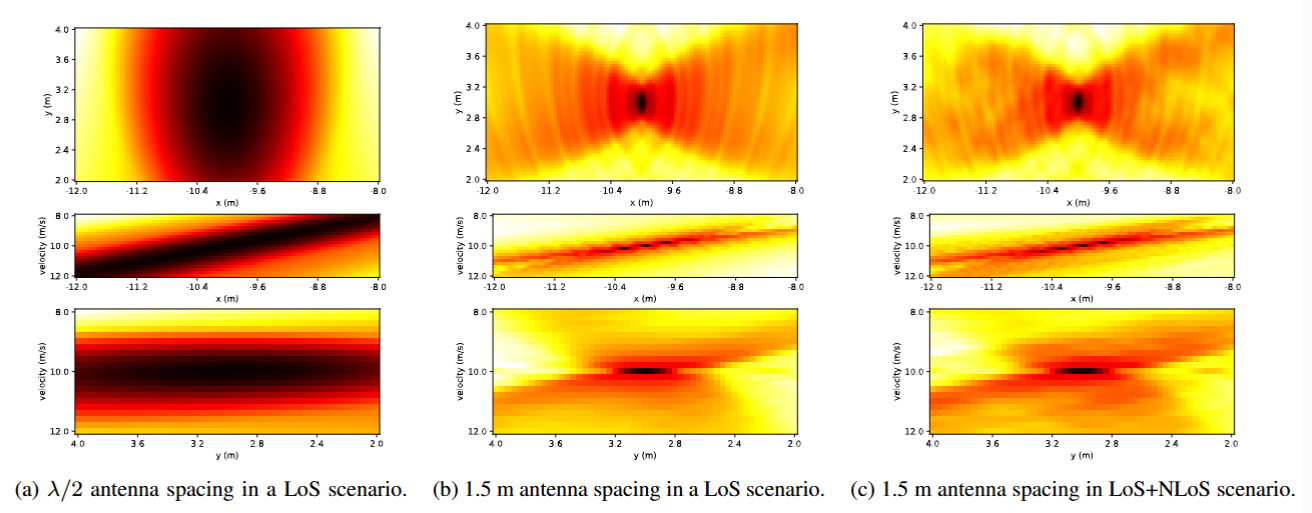
\includegraphics[width=0.8\linewidth]{figures(is_driver)/fig3.png}
\caption{图 3：在远场和近场场景中定位移动设备。(a) LoS 场景下的 $\lambda/2$ 天线间距。(b) LoS 场景下的 1.5 m 天线间距。(c) LoS+NLoS 场景下的 1.5 m 天线间距。在每个子图中，大面积黑色区域意味着定位不可行。小黑点表示车辆可以被准确定位。}
\label{fig:3}
\end{figure}

为了展示天线间距与方程 (4) 可解性之间的关系，让我们以图 2 中的情况为例。假设载波频率 $f=1890$ MHz。发射机（手机）的起始位置为 $(x_{0},y_{0})=(-10.0,3.0)$。速度为 $v=10.0$ m/s。探测器和发射机处于相同高度（即 $z=0$ 和 $\hat{z}=0$）。探测器的天线数量 $M=4$。天线间距为半波长 $(\lambda/2)$。进一步假设发射机和探测器之间仅存在 LoS 路径（即没有 NLoS 路径）。在这种设置下，我们模拟 $M$ 个天线的信道（即 $h_{i}, i=1,2,\dots,N_{s}$），然后求解方程 (4) 以找到发射机的初始位置。图 3a 显示了对方程 (4) 最佳解的穷举搜索结果。显然，当天线间距较小时，很难找到方程 (4) 的最佳解。

为了使问题可解，我们通过增加探测器的天线间距将远场定位问题转化为近场定位问题。具体而言，我们将天线间距设置为 1.5 m。图 3b 显示了对方程 (4) 最佳解的穷举搜索结果。可以清楚地看到，可以找到最佳解，并且相应的 $\hat{x}_{0}^{*}$、$\hat{y}_{0}^{*}$ 和 $\hat{v}^{*}$ 值可以被准确估计。

在上述案例中，我们假设信道只有 LoS 路径（即无 NLoS 路径）。一个自然的问题是，当信道具有不可忽略的 NLoS 路径时，问题是否可解。为了探索这个问题的答案，我们考虑发射机和探测器之间既有 LoS 又有 NLoS 路径的情况。LoS 路径强度为 1；三条 NLoS 路径的强度为 [0.5, 0.25, 0.125]。这三条 NLoS 路径是由发射机周围的三个物体引起的，坐标偏移量为 (2,0)、(0,1) 和 (1,2)。图 3c 显示了数值结果。可以看到，$\hat{x}_{0}^{*}$、$\hat{y}_{0}^{*}$ 和 $\hat{v}^{*}$ 的最佳值仍然可以被清晰地识别。这可以归因于 LoS 和 NLoS 路径随时间通常是不相关的。

\subsection{天线高度的影响}
方程 (4) 中的问题涉及四个优化变量 $(\hat{x}_{0}, \hat{y}_{0}, \hat{v}, \hat{z})$，导致寻找其最佳变量时面临计算挑战。对于 PhoLoc，确定车辆中手机的相对位置不需要天线高度信息。因此，我们研究天线高度 $z$ 对其他变量（即 $x_{0}$ 和 $y_{0}$）估计的影响。如果这些变量的估计对 $z$ 不敏感，我们可以在方程 (4) 中用估计值替换它。这样做将把优化搜索空间从四维减少到三维，从而减少所需的计算量。

对于私家车，轿车的平均高度约为 1.4 m，SUV 的平均高度约为 1.9 m，皮卡的平均高度约为 1.9 m。如果我们将 PhoLoc 的天线高度固定为 1.65 m，那么方程 (4) 中的高度误差在大多数情况下应小于 0.5 m。因此，我们使用 0.5 m 作为天线高度误差的上限，以研究其对相关值和其他参数估计的影响。

考虑如图 2 所示的四天线探测器，参数与 III-B 节中列出的相同。探测器有四个线性天线，间距为 1.5 m。在这种情况下，我们研究天线高度误差（$z$ 的误差）对 $(x_{0},y_{0},v)$ 估计的影响，以及其对相关结果的影响。

图 4 展示了我们的数值结果。很明显，$x_{0}$、$y_{0}$ 和 $v$ 的搜索在 LoS 和 NLoS 场景中均对天线高度误差不敏感。天线高度误差对 $x_{0}$ 和 $v$ 的估计影响可以忽略不计。它对 $y_{0}$ 的估计有轻微影响。$z$ 的 0.5 m 误差将引入 0.04 m 的 $y$ 误差，这在实践中是可以容忍的。

% [图片占位]
\begin{figure}[htbp]
\centering
% \includegraphics[width=0.8\linewidth]{figures(is_driver)fig4.png}
\caption{图 4：仰角误差对其他参数估计的影响。左上：对相关值的影响；右上：对 $x_{0}$ 估计的影响；左下：对 $y_{0}$ 估计的影响；右下：对 $v$ 估计的影响。}
\label{fig:4}
\end{figure}

为了理解为什么 $(x_{0},y_{0},v)$ 的估计对 $z$ 的误差具有鲁棒性，让我们关注方程 (3) 中的平方根项。在实践中，由于 $(\hat{x}_{0}+\hat{v}(t_{i}-t_{0})-a_{m})^{2}+\hat{y}_{0}^{2}\gg z^{2}$，去除 $z$ 对最终结果的影响可以忽略不计，如图 4 所示。因此，我们重新定义导向矢量 $b_{i}=[b_{1i},b_{2i},...,b_{Mi}]$ 的元素如下：
\begin{equation}
b_{mi}=e^{-j\frac{2\pi f}{c}\sqrt{(\hat{x}_{0}+\hat{v}(t_{i}-t_{0})-a_{m})^{2}+\hat{y}_{0}^{2}}}
\end{equation}
去除 $z$ 将显著减少寻找 $(x_{0},y_{0},v)$ 最佳值的优化空间，从而减少 PhoLoc 的计算量。

\subsection{速度变化的影响}
我们要找到移动设备位置的模型基于车辆行驶速度恒定的假设。为了满足这一假设，PhoLoc 不应安装在靠近十字路口或停车标志的位置。相反，它应安装在车辆直线平稳行驶的路段。作为旨在协助交通管理部门实施安全政策的路侧检测设备，放置在这些位置并不是过分的要求。

在本部分中，我们研究车辆速度变化对其位置估计的影响。我们考虑两种最常见的情况：车辆加速和车辆制动。为了尽量减少各种速度的影响，我们不估计手机的起始位置。相反，我们估计手机轨迹与 y 轴相交时的中间位置（见图 2）。由于很难通过解析方法表征速度变化的影响，我们再次诉诸数值方法。我们考虑 III-B 节中描述的场景。当 $x\in[-15,15]$ 时，探测器收集来自发射机（车内手机）的无线电信号。车辆的移动距离建模为 $d=vt+\frac{1}{2}at^{2}$，其中 $v\in\{10,20,30\}$，$a$ 是车辆的加速度，范围从 $-2~m/s^{2}$ 到 $2~m/s^{2}$。

图 5 描绘了 LoS 和 NLoS 场景中 $x$（手机的估计水平坐标）和 $y$（手机的估计垂直坐标）的估计误差。图中离散的估计误差源于固定的搜索步长，即 $x$ 为 0.01 m，$y$ 为 0.001 m。可以看出，在 LoS 和 NLoS 场景中，$x$ 的估计误差均小于 0.04 m。还可以看出，在两种场景中，$y$ 的估计误差均小于 0.005 m。数值结果（尽管来自单个案例研究）表明，所提出的方法对车辆加速和制动具有鲁棒性。

% [图片占位]
\begin{figure}[htbp]
\centering
% \includegraphics[width=0.8\linewidth]{figures(is_driver)fig5.png}
\caption{图 5：车辆加速度对 LoS 和 NLoS 两种场景下 $x$ 和 $y$ 估计的影响。}
\label{fig:5}
\end{figure}

在实践中，PhoLoc 仅在手机处于其附近时收集蜂窝信号进行定位。信号收集的持续时间通常小于 2 秒。在如此短的时间内，有许多路段车辆直线平稳行驶，速度变化小于 $2~m/s^{2}$。然而，车辆可能不仅仅是在加速或制动。速度变化仍然是 PhoLoc 估计误差的主要来源。

\section{设计}

\subsection{基本思路}
PhoLoc 旨在确定车辆驾驶员是否正在通话。为此，它需要知道手机在车内的相对位置，而不是其绝对位置。为了找出手机的相对位置，PhoLoc 配备了两个传感器：i) 一个激光雷达传感器，和 ii) 一个多天线无线电接收机。

激光雷达传感器主要有两个用途。首先，它记录车辆最初被检测到（即车辆前端被检测到）的时刻。我们将此时刻记为 $t_{s}$，它将用于计算手机的相对水平位置。其次，它测量自身与车辆一侧（左侧或右侧）之间的距离。我们将测量距离记为 $y_{s}$，它将用于推断手机的相对垂直位置。$y_{s}$ 的图示见图 1。

多天线无线电接收机将用于窃听手机发射的蜂窝无线电信号。我们增加其天线间距（实验中为 5 英尺），将远场定位问题转化为近场定位问题。然后，基于窃听到的蜂窝信号，它通过求解方程 (4) 中的问题来估计 $(x_{0},y_{0},v)$。结合两个传感器的测量结果，车内手机的相对位置（记为 $(\Delta x,\Delta y)$）可以计算如下：
\begin{subequations}
\begin{align}
\Delta x &= (t_{s}-t_{0})v-x_{0}, \\
\Delta y &= (y_{0}-y_{s}),
\end{align}
\end{subequations}
其中 $x_{0}, y_{0}, v$ 和 $t_{0}$ 获自多天线无线电探测器，而 $t_{s}$ 和 $y_{s}$ 获自激光雷达传感器。

\subsection{无 CSI 的手机定位}
\textbf{挑战与方法}。求解方程 (4) 中的问题以获得 $(x_{0},y_{0},v)$ 需要时刻 $t_{i}, i=0,1,2,\dots$ 的信道知识 $\vec{h}_{i}$。然而，由于 PhoLoc 充当窃听者并且不与手机进行直接通信，因此 PhoLoc 很难估计手机与自身之间的信道系数。这是因为估计信道系数需要嵌入在手机信号帧中的解调参考信号的知识。它还需要补偿每个信号帧的时间和频率偏移。这些要求给 PhoLoc 的设计带来了巨大的挑战。即使可能，估计信道系数也会给 PhoLoc 的实现带来令人望而生畏的计算要求。值得注意的是，对于 PhoLoc 来说，与手机同步比与基站同步要困难得多。这是因为基站周期性地广播 PSS 和 SSS，但手机不广播此类同步信号。

为了应对这一挑战，我们要重新审视方程 (4) 中的问题表述，旨在消除对信道知识的需求。基于方程 (2) 和方程 (3)，可以看出方程 (4) 中的相关性（内积）是利用不同天线元件上的信号相位差。幸运的是，天线上的信号相位差可以基于接收到的基带信号进行估计，既不需要时间/频率同步，也不需要信道估计。受此观察启发，我们将提出一种实用方案来估计大间距天线元件上的信号相位差。

为了估计 PhoLoc 处的相对信号相位，还存在另一个源于手机信号时变频率的挑战。基站及其服务的手机工作在主从模式。基站动态分配一个或多个资源块（12 个 OFDM 子载波 $\times$ 7 个 OFDM 符号）用于其服务手机的上行链路传输，以提高频谱效率。分配给手机的资源块随时间快速变化。图 6 显示了真实 T-Mobile 手机在进行语音通话时的信号频率示例。可以看出，信号频率不是固定的，而是快速变化的。为了应对这一挑战，问题表述中需要考虑时变信号频率；并且应消除其影响。

% [图片占位]
\begin{figure}[htbp]
\centering
% \includegraphics[width=0.8\linewidth]{figures(is_driver)fig6.png}
\caption{图 6：手机信号频率和时间戳示例。该手机使用 T-mobile 网络，工作在两个频段：1720 MHz 和 1890 MHz。}
\label{fig:6}
\end{figure}

\textbf{手机定位}。基于第三节的结果，我们提出了一种手机定位方案，既不需要时间/频率同步也不需要信道估计，同时考虑了手机信号的时变频率。图 7 描绘了我们提出的手机定位方案的框图，该方案由以下三个组件组成。

% [图片占位]
\begin{figure}[htbp]
\centering
% \includegraphics[width=0.8\linewidth]{figures(is_driver)fig7.png}
\caption{图 7：PhoLoc 信号采集方案示意图。}
\label{fig:7}
\end{figure}

\begin{itemize}
    \item \textbf{手机信号搜索}。当车辆接近时，PhoLoc 首先需要弄清楚两个问题：i) 车内是否有活跃的电话通话？ii) 电话通话使用的上行链路频率信道是什么？为了找到这两个问题的答案，PhoLoc 监测所有可能的上行链路蜂窝信道（例如 1.5 GHz-3.6 GHz）上的无线电信号的功率水平和频谱模式。如果周期性地检测到高于预定义功率阈值的蜂窝信号，则认为车内有活跃的电话通话，并可以相应地识别其频率信道。这种方法在实践中是有效的，原因有二。首先，在我们的问题设置中，感兴趣的车辆非常靠近 PhoLoc（例如几十米）。因此，如果车内有活跃的手机，PhoLoc 将持续观察到明显强的手机信号。此外，由于车辆正驶向 PhoLoc，PhoLoc 观察到的手机信号功率在不断增加。这些特征使得 PhoLoc 很容易检测车内的活跃电话通话及其关联的频率信道。其次，得益于软件无线电（SDR）技术的进步，可以快速实现多信道的频谱监测。由于 PhoLoc 只需要少量手机信号数据进行定位（例如在我们的实验中信号收集不到 2 秒），当车辆驶向 PhoLoc 时，PhoLoc 有足够的时间监测所有上行链路蜂窝信道的频谱。此功能使 PhoLoc 能够定位车内不同频段上的多个手机。
    
    \item \textbf{FFT}。此模块将手机信号从时域转换为频域。PhoLoc 对此模块使用 30.72 MHz 采样率和 2048 个 FFT 点。我们强调，PhoLoc 在 FFT 操作之前没有时间/频率估计和补偿。
    
    \item \textbf{手机信号提取}。手机在进行语音通话时可能会使用一个或多个资源块进行数据传输。当手机使用多个资源块进行传输时，其宽带信号会模糊 PhoLoc 天线上的相位差。因此，我们选择一部分强的相邻子载波进行信号相位差估计。设 $y_{mik}$ 为 FFT 结果，其中 $m$ 是天线索引，$i$ 是数据样本索引，$k$ 是子载波索引。设 $\mathcal{R}_{i}$ 为选择用于相位估计的子载波子集。然后，我们令
    \begin{equation}
    \mathcal{R}_{i}=\{k:|k-k_{max}|<N_{RB}/2,|y_{mik}|>\eta y_{max}\}
    \end{equation}
    其中 $N_{RB}$ 是资源块中的子载波数（4G LTE 中 $N_{RB}=12$）；$k_{max}$ 和 $y_{max}$ 分别是最强子载波的索引和幅度；$\eta$ 是经验选择的阈值（在我们的实验中 $\eta=0.3$）。选择子载波子集后，我们构造信号向量如下：
    \begin{equation}
    \vec{s}_{i}=[s_{1i},s_{2i},\dots,s_{Mi}]
    \end{equation}
    其中
    \begin{equation}
    s_{mi}=\frac{\sum_{k\in\mathcal{R}_{i}}y_{mik}}{|\sum_{k\in\mathcal{R}_{i}}y_{mik}|}
    \end{equation}
    归一化操作背后的原理是信号相位携带感兴趣的信息，而信号幅度则不携带。$\vec{s}_{i}$ 的对应频率可以近似写为：
    \begin{equation}
    f_{i}=f_{c}+\frac{\sum_{k\in\mathcal{R}_{i}}k}{|\mathcal{R}_{i}|}\frac{f_{s}}{N_{fft}}
    \end{equation}
    其中 $|\cdot|$ 是集合的基数，$f_{c}$ 是中心频率，$f_{s}$ 是信号采样率，$N_{fft}$ 是 FFT 大小。在 PhoLoc 中，$f_{s}=30.72$ MHz 且 $N_{fft}=2048$。有了信号向量 $\vec{s_{i}}$、其频率 $f_{i}$ 和其时间戳 $t_{i}$，我们将方程 (4) 中的定位问题重构如下：
    \begin{equation}
    [\hat{x}_{0}^{*},\hat{y}_{0}^{*},\hat{v}^{*}]= \arg \max_{\hat{x}_{0},\hat{y}_{0},\hat{v}}\sum_{i=0}^{N_{s}}|\vec{s}_{i}\vec{b}_{i}^{H}|,
    \end{equation}
    其中导向矢量 $\vec{b}_{i}=[b_{1i},b_{2i},\dots,b_{Mi}]$ 的元素重写为：
    \begin{equation}
    b_{mi}=e^{-j\frac{2\pi f_{i}}{c}\sqrt{(\hat{x}_{0}+\hat{v}(t_{i}-t_{0})-a_{m})^{2}+\hat{y}_{0}^{2}}}
    \end{equation}
\end{itemize}

对于图 7 中的操作，我们有以下两点说明。
\textbf{备注}。对于上述用于手机定位的信号采集，我们有两点备注。首先，在 FFT 之前没有频率和时间偏移补偿，估计的频域符号（图 7 中 FFT 的输出）将不遵循经典的无线通信模型 $y=hx+n$，其中 $y$ 是接收信号，$h$ 是信道系数，$x$ 是传输信号。它们也不能代表真实的信道。然而，频域信号 $(\vec{s}_{i})$ 的相位差是其信道相位差的近似值。其次，如图 7 所示，PhoLoc 不同于典型的多天线接收机。它没有帧检测、频率/时间估计和补偿以及信道估计。去除这些信号处理模块极大地简化了 PhoLoc 的实现。

\subsection{激光雷达和无线电接收机的联合优化}
使用方程 (6) 估计 $(\Delta x,\Delta y)$ 面临两个挑战。首先，无线电接收机和激光雷达传感器的数据采样率非常不同。根据 3GPP，VoIP 数据包间隔高达 40 毫秒，产生 25 Hz 的数据采样率。如果激光雷达以 VoIP 数据包速率测量距离，当车辆以 $25~m/s$ 行驶时，测量误差可能高达 1 米。因此，无线电接收机和激光雷达传感器的测量数据应针对手机定位进行同步。其次，根据方程 (6a)，如果 $v$ 不是常数，则 $\Delta x$ 的估计将产生累积误差。为了最小化累积误差，我们使用近场定位算法来估计时刻 $t_{s}$ 而不是时刻 $t_{0}$ 的手机位置。这样做不仅解决了低数据包率问题，而且减少了由不准确速度估计引起的累积误差。

数学上，我们定义 $(x_{p},y_{p})$ 为时刻 $t_{s}$（即车辆前端刚刚被激光雷达检测到）的手机坐标。根据方程 (6)，我们有 $\Delta x=-x_{p}$ 和 $\Delta y=y_{p}-y_{s}$。然后，基于方程 (11)，我们将导向矢量 $\vec{b}_{i}=[b_{1i},b_{2i},\dots,b_{Mi}]$ 的元素重写如下：
\begin{equation}
b_{mi}=e^{-j\frac{2\pi f_{i}}{c}\sqrt{(-\Delta\hat{x}+\hat{v}(t_{i}-t_{s})-a_{m})^{2}+(\Delta\hat{y}+y_{s})^{2}}}
\end{equation}
其中 $\Delta x$, $\Delta y$ 和 $y_{s}$ 如图 1 所示。最后，手机定位问题可以表示为：
\begin{equation}
[\Delta\hat{x}^{*},\Delta\hat{y}^{*},\hat{v}^{*}]= \arg \max_{\Delta\hat{x},\Delta\hat{y},\hat{v}}\sum_{i}|\vec{s}_{i}\vec{b}_{i}^{H}|
\end{equation}
其中 $\vec{s}_{i}$ 在方程 (8) 中给出，$\vec{b}_{i}$ 在方程 (12) 中给出。

为了求解方程 (13)，需要搜索三个变量。对于大多数私家车（轿车和 SUV），其长度小于 5 米，宽度小于 2 米。因此，我们经验性地将 $\Delta\hat{x}$ 的搜索范围设置为 [0, 5]，将 $\Delta\hat{y}$ 的搜索范围设置为 [-0.5, 2.5]。一个问题是 $\hat{v}$ 的范围是什么。在实践中，同一位置的车辆速度可能非常不同（例如，从 20 mph 到 45 mph）。为了减少搜索空间，我们利用激光雷达的数据。设 $\tau$ 为车辆通过激光雷达的时间持续时间。由于私家车的平均长度为 4.6 米，我们设置参考速度为 $v_{ref}=4.6/\tau$。然后，我们经验性地将 $\hat{v}$ 的搜索范围设置为 $[0.7v_{ref}, 1.3v_{ref}]$。由于方程 (13) 中的搜索问题天然适合并行计算，我们在实验中使用穷举搜索来追求其最佳解。通过在 i7-10700 CPU 上使用 8 个线程，在我们的实验中找到最佳解所需的时间不到 2 秒。

设 $c^{*}$ 为最佳归一化相关值。那么，它可以写为：
\begin{equation}
c^{*} = \frac{1}{N_{s}+1} \sum_{i=0}^{N_{s}} |\vec{s}_{i}\vec{b}_{i}^{H}|_{\Delta\hat{x}=\Delta\hat{x}^{*},\Delta\hat{y}=\Delta\hat{y}^{*},\hat{v}=\hat{v}^{*}},
\end{equation}
其中 $M$ 是天线数量，$N_{s}+1$ 是数据样本的数量。

\subsection{整合}
图 8 描绘了 PhoLoc 检测驾驶员通话违规的总体框图。部分步骤描述如下。

% [图片占位]
\begin{figure}[htbp]
\centering
% \includegraphics[width=0.8\linewidth]{figures(is_driver)fig8.png}
\caption{图 8：PhoLoc 检测通话违规的决策树。}
\label{fig:8}
\end{figure}

\textbf{蓝牙免提检测}。在一些国家和地区，驾驶时使用基于蓝牙的免提通话是被允许的。幸运的是，由于蜂窝信号和蓝牙信号的频段不同，路侧基础设施可以很容易地检测到免提通话。图 9 显示了路侧无线电接收机（5 米距离）从一辆丰田车收集的蓝牙信号。可以看出，当车辆蓝牙处于不同模式时，流量强度有显著差异。还可以看出，蓝牙功率随距离迅速衰减。这些观察结果表明，通过监测蓝牙的流量强度和频率，可以可靠地检测到使用蓝牙进行免提通话。

% [图片占位]
\begin{figure}[htbp]
\centering
% \includegraphics[width=0.8\linewidth]{figures(is_driver)fig9.png}
\caption{图 9：不同模式下的蓝牙流量强度和相对信号功率。}
\label{fig:9}
\end{figure}

\textbf{决策制定}。在计算出方程 (13) 和方程 (14) 的最佳值后，PhoLoc 检测驾驶员通话违规如下：
\begin{equation}
D = \begin{cases} 
\text{violation of phone call} & \text{if } \Delta x^{*}\ge x_{th}, \Delta y^{*}\le y_{th}, c^{*}\ge c_{th}, \\
\text{no violation} & \text{otherwise},
\end{cases}
\end{equation}
其中 $x_{th}$, $y_{th}$ 和 $c_{th}$ 是用于做出决策的阈值。阈值 $c_{th}$ 可用于平衡 PhoLoc 的误报率和漏报率。在我们的实验中，我们经验性地设置 $c_{th}=0.61$。对于 $x_{th}$ 和 $y_{th}$，PhoLoc 并不简单地将它们设置为固定值。相反，它首先通过 $L_{veh}=\hat{v}^{*}\tau$ 估计车辆长度，其中 $\tau$ 是激光雷达传感器检测到车辆的持续时间。根据车辆长度，PhoLoc 经验性地设置它们的值如下：如果 $L_{veh}\le4.9$ m，则 $(x_{th},y_{th})=(2.70,0.93)$；否则 $(x_{th},y_{th})=(2.80,0.96)$。注意 PhoLoc 仅针对私家车（例如轿车和 SUV）进行检测。可以利用更复杂的方法来为这三个阈值设定值。

\section{实验评估}

\subsection{实现}
图 10 展示了我们的 PhoLoc 原型，它是使用 USRP N310、激光雷达、PC 和四个 LTE 天线构建的。

% [图片占位]
\begin{figure}[htbp]
\centering
% \includegraphics[width=0.8\linewidth]{figures(is_driver)fig10.png}
\caption{图 10：天线升起（左）和天线置地（右）的 PhoLoc 照片。}
\label{fig:10}
\end{figure}

\textbf{无线电设备}。我们使用 USRP N310 设备构建了 PhoLoc 无线电接收机的原型，该设备具有 4 个通道，频率范围从 10 MHz 到 6 GHz，支持 100 MHz 瞬时带宽。USRP 设备通过 10 Gigabit SFP+ 以太网与 Dell XPS 台式机（i7-10700 CPU，16 G RAM）连接。四个带有 8 英尺电缆的低成本 LTE 天线安装在 USRP N310 上用于蜂窝信号接收。

\textbf{激光雷达传感器}。我们使用 MakerFocus TFmini-s 模块（亚马逊售价 43 美元 [29]）作为 PhoLoc 的激光雷达传感器，以测量其自身与车辆之间的距离。根据其手册，该模块提供 0.1 m-12 m 的测量范围，测量频率为 1000 Hz。其距离分辨率为 1 cm，测距精度为 6 cm 或测量距离的 1\%。我们的实验室测试表明，最大测量频率为 876 Hz。激光雷达传感器通过 USB 接口与同一台 Dell 计算机连接，它们的通信协议是 UART。

\textbf{软件}。我们使用 GNU Radio 树外（OOT）模块 [30] 实现了 PhoLoc 的软件。图 7 中的信号处理模块是用 C++ 实现的。图 7 中的每个模块都在单独的线程中实现以进行并行计算，从而实现实时计算。从激光雷达传感器获取的距离数据被发送到 GNU Radio [31] 进行数据融合。所有无线电和激光雷达数据样本均使用无线电采样率（30.72 MHz）打上时间戳。

\textbf{实验设置}。如图 10 所示，我们的实验考虑了两种天线配置：i) 天线固定在 3.5 英尺高度，和 ii) 天线放置在地面上。三人（两名驾驶员和一名乘客）参与了我们的实验。驾驶员或乘客手持 T-Mobile 手机进行语音通话（通过 VoLTE），将手机放置在三个不同位置：左耳、右耳和嘴前，如图 11 所示。另一部 T-Mobile 手机也放置在车内播放流媒体音乐。它作为一个潜在的干扰源，产生除 VoIP 流量之外的突发数据流量。我们注意到，我们并没有刻意关闭这两部手机其他应用程序产生的其他数据流量。在测试期间，车窗保持关闭。在整个实验过程中，我们使用了两辆车进行测试：丰田 RAV4 和丰田凯美瑞。PhoLoc 在检测通话违规时没有车辆的先验知识。

% [图片占位]
\begin{figure}[htbp]
\centering
% \includegraphics[width=0.8\linewidth]{figures(is_driver)fig11.png}
\caption{图 11：电话呼叫者位于不同的座位。}
\label{fig:11}
\end{figure}

\subsection{实验室验证}
在进行路测之前，我们首先在实验室验证所提出的近场定位方案。我们将 PhoLoc 和一部手机放置在实验室地板上。PhoLoc 有四个天线，天线间距为 1 m。天线坐标为 (-1.5, 0), (-0.5, 0), (0.5, 0), 和 (1.5, 0)。我们将一部正在进行语音通话的 T-Mobile 手机从 (-2.5, 0) 移动到 (2.5, 0)，步长为 5 cm，如图 12 所示。共收集了 101 个数据样本。基于收集的数据，我们使用方程 (10) 中的公式搜索手机的起始位置（即 $x_{0}$ 和 $y_{0}$）。图 13 显示了搜索结果的逆热图。估计的起始位置为 (-2.520, 0.995)。这意味着 $x_{0}$ 的估计误差为 2 cm，$y_{0}$ 的估计误差为 0.5 cm。图 13 还显示了沿 x 和 y 轴的归一化相关性。可以看出，沿 x 和 y 轴的相关峰值都很明显。结果揭示了所提出的近场定位方案的鲁棒性。

% [图片占位]
\begin{figure}[htbp]
\centering
% \includegraphics[width=0.8\linewidth]{figures(is_driver)fig12.png}
\caption{图 12：实验室验证的实验设置。(a) 设置。(b) 实验设置照片。}
\label{fig:12}
\end{figure}

% [图片占位]
\begin{figure}[htbp]
\centering
% \includegraphics[width=0.8\linewidth]{figures(is_driver)fig13.png}
\caption{图 13：寻找手机起始位置的实验结果。[左]：PhoLoc 生成的逆相关热图。[右]：沿 x 和 y 轴的归一化相关性。}
\label{fig:13}
\end{figure}

\subsection{路测案例研究}
我们将 PhoLoc 部署在路边，如图 10 所示。四个天线被提升到 3.5 英尺（1.07 m），天线间距为 5 英尺（1.524 m）。激光雷达传感器放置在四个天线的正中间，面向道路。一个人驾驶车辆（丰田 RAV4）从右向左行驶。驾驶员正在通话，其手机使用 T-Mobile 4G 服务。他将手机放在左耳上，没有使用蓝牙进行免提连接。车辆的速度计读数为 20 mph。

\textbf{激光雷达测量}。图 14（左）显示了激光雷达的数据。PhoLoc 每毫秒读取一次激光雷达的测量值。激光雷达传感器检测到车辆的持续时间为 $\tau=0.47$ s。因此，车辆速度估计为 $4.6/0.47=9.78~m/s$，其中 4.6 是市场上所有私家车的平均长度。根据估计的速度，我们将 $v$ 的搜索范围设置为 $[0.70\times9.78, 1.3\times9.78]$，步长为 $0.02~m/s$。最佳值结果为 $9.47~m/s$，非常接近估计值。然后，让我们放大图 14（左）中激光雷达测量的距离。可以看出，测量距离从 2.8 m 变化到 3.0 m。为了减少测量误差，我们排除了两侧的测量值，并对其余测量值取平均。结果用作 $y_{s}$，在本例中为 2.86 m。

% [图片占位]
\begin{figure}[htbp]
\centering
% \includegraphics[width=0.8\linewidth]{figures(is_driver)fig14.png}
\caption{图 14：激光雷达距离输出（左），信号样本间隔（中），信号频率（右）。}
\label{fig:14}
\end{figure}

\textbf{信号间隔和频率}。图 14（中）显示了 PhoLoc 测量的手机传输的信号间隔。可以看出，在大多数时间里，信号时间间隔为 40 ms。这与 VoIP 标准一致。对于这种情况，PhoLoc 使用了 1.49 s 时间持续的信号样本来估计手机位置，对应于车辆 14 m 的移动距离。图 14 中的右图绘制了手机信号的频率。它以 1725 MHz 为中心，跨度超过 20 MHz。可以看出，手机数据包的传输频率随时间快速变化。这是因为手机的传输频率由其关联的基站动态调度。

\textbf{信号幅度和相位}。图 15a 显示了接收机四个天线的信号幅度比。图 15b 显示了它们的相位差。可以看出信号幅度非常动态。我们对信号幅度进行归一化，以便每个信号样本的相位携带相同的权重。虽然相位看起来嘈杂，但它实际上带有某种由车辆移动引起的模式。这种固有模式在推断手机位置中起着关键作用。

% [图片占位]
\begin{figure}[htbp]
\centering
% \includegraphics[width=0.8\linewidth]{figures(is_driver)fig15.png}
\caption{图 15：从无线电接收机收集的信号样本。(a) 四个天线的信号幅度比。(b) 四个天线的信号相位差。}
\label{fig:15}
\end{figure}

\textbf{相关热图}。基于从无线电和激光雷达收集的数据，PhoLoc 进行了暴力搜索以找到方程 (13) 的最佳解。得到的最佳值为 $\Delta\hat{x}^{*}=2.09$ m, $\Delta\hat{y}^{*}=0.46$ m, $\hat{v}^{*}=9.48~m/s$, 和 $c^{*}=0.7$。图 16a 显示了 PhoLoc 生成的相关逆热图，其中暗像素代表高相关性，而亮像素代表低相关性。逆热图清楚地显示了其峰值，集中在一个小区域内。

\textbf{决策和估计误差}。基于优化后的车辆速度，车辆长度估计为 $L_{veh}=\hat{v}^{*}\tau=9.48\times0.47=4.45$ m，其中 $\tau$ 是激光雷达检测到车辆的时间持续时间。由于 $L_{veh}\le4.9$，我们根据预定义标准令 $(x_{th},y_{th})=(2.7,0.93)$。然后，根据方程 (15)，本例中的手机位置将被分类为驾驶员座位。我们的手动测量表明 $\Delta x=2.25$ m 和 $\Delta y=0.36$ m。虽然它们不是很准确，但我们将其作为地面实况。那么，PhoLoc 在这种情况下的误差为 $\epsilon_{x}=16$ cm 和 $\epsilon_{y}=10$ cm。

\textbf{天线高度的影响}。此前我们通过仿真表明 PhoLoc 对天线高度不敏感。现在我们使用实验来测试这一假设。我们重复了上述案例研究，但将天线放置在地面上，如图 10 所示。此设置在搜索手机位置时引入了约 1.5 m 的天线高度误差 $z$。图 16b 显示了 PhoLoc 生成的热图。比较图 16 中的两幅图，可以看出天线高度的大误差确实降低了 PhoLoc 的性能。因此，在接下来的实验中，我们使用四个天线固定在 3.5 英尺高度的实验设置。

% [图片占位]
\begin{figure}[htbp]
\centering
% \includegraphics[width=0.8\linewidth]{figures(is_driver)fig16.png}
\caption{图 16：PhoLoc 天线高度不同时生成的逆相关热图。(a) 3.5 ft 天线高度。(b) 地面天线。}
\label{fig:16}
\end{figure}

\subsection{天线间距的影响}
我们重复了上述案例研究中描述的实验，但 PhoLoc 具有不同的天线间距：2 ft, 3 ft, 4 ft, 和 5 ft。对于每种情况，我们进行了 15 次测试。驾驶员相同，车辆相同。驾驶员将手机放在左耳上。车辆速度约为 20 mph。图 17 显示了 PhoLoc 具有不同天线间距时的逆热图示例。图 18 显示了每种情况下前五次测试的测量结果。很明显，当天线间距较小时，PhoLoc 表现不佳。增加天线间距往往会提高 PhoLoc 的性能。在 15 次测试中，$(\Delta x,\Delta y)$ 的标准偏差在 2 ft 间距情况下为 (0.11, 0.72)，在 3 ft 间距情况下为 (0.10, 0.16)，在 4 ft 间距情况下为 (0.12, 0.10)，在 5 ft 间距情况下为 (0.06, 0.08)。

一个问题是更大的天线间距是否总是更好。我们的观察是否定的。更大的天线间距要求车辆在更长的距离内保持恒定速度。此外，车辆的轨迹应与天线阵列更严格地平行。这意味着具有更大天线间距的 PhoLoc 对车辆的速度变化和方向误差更敏感。此外，它需要更多的部署空间。基于上述考虑，我们建议 PhoLoc 使用 5 ft 作为其天线间距。

% [图片占位]
\begin{figure}[htbp]
\centering
% \includegraphics[width=0.8\linewidth]{figures(is_driver)fig17.png}
\caption{图 17：PhoLoc 使用不同天线间距时生成的逆相关热图。(a) 2 ft 天线间距。(b) 3 ft 天线间距。(c) 4 ft 天线间距。(d) 5 ft 天线间距。}
\label{fig:17}
\end{figure}

% [图片占位]
\begin{figure}[htbp]
\centering
% \includegraphics[width=0.8\linewidth]{figures(is_driver)fig18.png}
\caption{图 18：PhoLoc 使用不同天线间距时的估计手机位置。}
\label{fig:18}
\end{figure}

\subsection{车辆速度的影响}
我们在不同的车辆速度下重复了上述测试：10 mph ($4.5~m/s$), 15 mph ($6.7~m/s$), 20 mph ($8.9~m/s$), 和 30 mph ($13.4~m/s$)。不幸的是，由于速度限制，我们不被允许以更高的速度进行测试。我们对每种情况进行了 20 次测试。在我们的测试中，天线间距为 5 ft，手机位于驾驶员的左耳上。图 19 显示了每种情况下逆热图的示例。图 20 显示了每种情况下前五次测试的结果。在所有测试中，$(\Delta x,\Delta y)$ 的标准偏差在 10 mph 情况下为 (0.24, 0.24)，在 15 mph 情况下为 (0.12, 0.25)，在 20 mph 情况下为 (0.12, 0.13)，在 30 mph 情况下为 (0.07, 0.14)。

基于实验结果可以得出两个观察结论：i) PhoLoc 在所有测试车辆速度下表现良好；ii) 较高的车辆速度往往提供更好的性能。第二个观察结果可归因于这样一个事实，即在实践中，车速较高时车辆速度更稳定。也就是说，$a/v$ 随着 $v$ 的增加而减小，其中 $v$ 是车辆速度，$a$ 是车辆加速度。

% [图片占位]
\begin{figure}[htbp]
\centering
% \includegraphics[width=0.8\linewidth]{figures(is_driver)fig19.png}
\caption{图 19：车辆以不同速度行驶时 PhoLoc 生成的逆相关热图。(a) 10 mph 速度。(b) 15 mph 速度。(c) 20 mph 速度。(d) 30 mph 速度。}
\label{fig:19}
\end{figure}

% [图片占位]
\begin{figure}[htbp]
\centering
% \includegraphics[width=0.8\linewidth]{figures(is_driver)fig20.png}
\caption{图 20：车辆以不同速度行驶时 PhoLoc 的结果。}
\label{fig:20}
\end{figure}

\subsection{驾驶员手持方式的影响}
在这项研究中，当驾驶员进行语音通话时，我们重复上述实验。我们考虑三种情况：i) 驾驶员将手机放在左耳上；ii) 驾驶员将手机放在嘴前；iii) 驾驶员将手机放在右耳上（见图 11）。对于每种情况，我们进行了 20 次测试。对于这些测试，天线间距为 5 ft，车辆速度约为 20 mph。图 21 显示了每种情况下前 10 次测试的结果。在所有测试中，当驾驶员将手机放在左耳上时，$(\Delta x,\Delta y)$ 的标准偏差为 (0.09, 0.17)；当驾驶员将手机放在嘴前时，标准偏差为 (0.13, 0.10)；当驾驶员将手机放在右耳上时，标准偏差为 (0.49, 0.41)。

显然，当手机在嘴前时 PhoLoc 性能最好，当手机在左耳时性能可接受，而当手机在右耳时性能较差。这是因为在前两种情况下，PhoLoc 有 LoS 路径到达手机，而在第三种情况下没有 LoS 路径到达手机。当驾驶员将手机放在耳朵上时，他的头部遮挡了信号，导致 PhoLoc 性能不佳。

% [图片占位]
\begin{figure}[htbp]
\centering
% \includegraphics[width=0.8\linewidth]{figures(is_driver)fig21.png}
\caption{图 21：手机处于不同位置时 PhoLoc 的结果。}
\label{fig:21}
\end{figure}

\subsection{车内手机位置的影响}
我们进行了测试以评估呼叫者位于车内不同座位时 PhoLoc 的性能。具体而言，我们考虑了呼叫者的四个位置：驾驶员座、副驾驶座、左后座和右后座。对于每种情况，我们对呼叫者的左耳进行了 10 次测试，对呼叫者的嘴前进行了 10 次测试，对呼叫者的右耳进行了 10 次测试。实验设置如图 11 所示。在这些测试中，车内同时有两人。与 V-F 节中的观察类似，当手机位于呼叫者左耳和嘴前时，PhoLoc 表现良好，但当手机位于右耳时，表现不佳。原因相同，即当手机在右耳时，呼叫者的头部遮挡了信号。解决此问题的一个简单方法是在路边部署两个 PhoLoc 设备：一个在车辆左侧，另一个在车辆右侧。因此，我们只展示手机位于呼叫者左耳和嘴前时的结果。图 22 显示了手机位于呼叫者左耳时四种情况的逆相关热图。图 23 展示了手机位于呼叫者左耳或嘴前时四种情况的结果。总体而言，当呼叫者在驾驶员座位时，$(\Delta x,\Delta y)$ 的标准偏差为 (0.15, 0.18)；在副驾驶座位时为 (0.21, 0.21)；在左后座时为 (0.11, 0.19)；在右后座时为 (0.28, 0.24)。

% [图片占位]
\begin{figure}[htbp]
\centering
% \includegraphics[width=0.8\linewidth]{figures(is_driver)fig22.png}
\caption{图 22：呼叫者位于不同座位且手持电话在左耳时 PhoLoc 生成的逆相关热图。(a) 驾驶员座。(b) 副驾驶座。(c) 左后座。(d) 右后座。}
\label{fig:22}
\end{figure}

% [图片占位]
\begin{figure}[htbp]
\centering
% \includegraphics[width=0.8\linewidth]{figures(is_driver)fig23.png}
\caption{图 23：当电话由车内不同座位的呼叫者拨打时 PhoLoc 的结果。}
\label{fig:23}
\end{figure}

\subsection{广泛的实验结果}
\textbf{驾驶员通话违规检测}。回想一下，我们的目标是检测车辆驾驶员的通话违规行为。总共，我们对车辆驾驶员正在通话的事件进行了 58 次测试。PhoLoc 对其中的 8 次做出了错误的决定，其中大多数对应于驾驶员将手机放在右耳的情况。因此，漏报率为 (8/58=) 13.8\%。另一方面，我们对电话是由乘客（在副驾驶座或后座）而不是驾驶员拨打的事件总共进行了 96 次测试。PhoLoc 对 4 次测试做出了错误的决定。因此，误报率为 $(4/96)=4.2\%$。此外，我们注意到，当乘客将手机放在右耳上时，方程 (14) 中的结果相关值通常小于阈值 $(c_{th}=0.61)$，因此，PhoLoc 不会对这些情况做出错误的决定。表 I 总结了 PhoLoc 的总体结果。

\textbf{手机/呼叫者车内位置分类}。PhoLoc 的一个自然扩展是对车内活跃电话呼叫者的位置进行分类：驾驶员座、副驾驶座、左后座或右后座。对于这个问题，我们假设在道路两侧部署了两个 PhoLoc 设备。我们使用上述测量结果来推断位置检测的准确性。具体而言，我们排除驾驶员或乘客将手机放在右耳的情况下的数据，因为这种情况可以由另一个 PhoLoc 设备处理。数据分析表明，在总共 103 次测试中，23 次测试产生的相关性小于 $c_{th}$（即 0.61）。因此，无效数据率为 $(23/103=)$ 22.3\%。在那些有效测量中，PhoLoc 在 69 次测试中找到了正确的位置。所以分类准确率为 $(69/80=)$ 86.3\%。表 I 总结了我们的总体结果。

% [表格占位]
\begin{table}[htbp]
\caption{表 I：PhoLoc 的总体性能。}
\centering
\begin{tabular}{|c|c|c|}
\hline
\textbf{驾驶员通话违规检测} & 误报率 (False positive rate) & $4.2\%$ \\
 & 漏报率 (False negative rate) & $13.8\%$ \\
\hline
\textbf{手机位置分类} & 无效数据比例 & $22.3\%$ \\
 & 分类准确率 & $86.3\%$ \\
\hline
\end{tabular}
\label{tab:1}
\end{table}

\section{局限性与讨论}

\textbf{计算高效算法}。为了找到手机的相对位置，我们将问题表述为优化问题，并采用暴力搜索来寻求其最佳解。虽然暴力搜索可以在几秒钟内完成，但仍需高效的求解算法。一种可能的方法是解耦 $\Delta x$, $\Delta y$ 和 $v$，以便可以通过 3 维 FFT 操作（遵循 Omega-K 算法 [32] 的思路）找到这三个变量的最佳值。

\textbf{其他手机使用违规行为}。驾驶员的手机使用违规行为包括打电话、发短信、浏览网站等。虽然 PhoLoc 是为检测驾驶员通话违规而设计和评估的，但它也可用于检测其他手机使用违规行为。例如，发一条短信时，手机的间歇信号传输将持续数秒。可以按照我们提出的方式收集和处理手机信号，以对车内的手机位置进行分类并检测驾驶员的手机使用违规行为。在未来的工作中，我们将使用手机发射的无线电信号来：i) 对用户的活动进行分类（例如发短信、浏览网页和听音乐），以及 ii) 估计其在车内的相对位置。基于分类和估计结果，我们将设计一种基于学习的方法来确定车内是否存在手机使用违规行为。

\textbf{车辆密集场景}。在道路车辆密集的场景中，PhoLoc 与目标车辆之间的 LoS 路径可能会被另一辆车阻挡。在这种情况下，单个 PhoLoc 探测器可能由于其激光雷达传感器的距离测量不准确而无法正常工作。鉴于激光雷达对车辆的有效测量时间短（小于 1 秒），可以通过在道路两侧部署多个 PhoLoc 探测器来缓解此问题。我们预计，增加路侧 PhoLoc 探测器的数量将显着提高检测车辆驾驶员手机使用违规行为的准确性。

\textbf{误差来源}。我们系统中定位误差的主要来源可归因于几个因素：(i) 不准确的无线电频率：PhoLoc 用于估计无线电信号波长的频率是来自多个子载波的平均值。无线电信号的载波频率是一个估计值，并不准确。(ii) 车辆速度的变化：在测量期间，车辆的速度可能不是恒定的。车辆速度的变化可能会导致 PhoLoc 的定位误差。(iii) 噪声和其他缺陷：PhoLoc 在 SDR 测试平台上实现了所提出的定位方法，该平台未针对带外干扰和噪声抑制进行优化。SDR 平台的噪声和其他缺陷导致了 PhoLoc 的定位误差。(iv) 激光雷达测量误差：由于车辆移动导致的激光雷达测量 $y_{s}$ 的变化，以及连续测量的 $y_{s}$ 的平均，是 PhoLoc 定位误差的另一个来源。

\section{相关工作}
我们回顾了两个领域的相关工作：分心驾驶检测和无线定位。

\textbf{基于摄像头的分心驾驶检测}。摄像头与基于 AI 的计算机视觉技术已被广泛研究，以监控车辆驾驶员的状态并检测其手机使用违规行为 [33], [4], [34]–[39]。然而，这些工作大多数要求摄像头安装在车内。因此，所提出的基于摄像头的检测系统主要限于私人使用（例如商用车辆）。最近，在路边部署高分辨率摄像头以检测分心驾驶员已成为执行驾驶安全相关法律的新方法 [2]。一些国家（如英国和奥地利）已经试验了这种方法，并证明了其在实践中的可行性 [2]。尽管计算机视觉取得了最新进展，但基于摄像头的方法在某些场景（例如黑暗和恶劣天气条件）中可能效果不佳，并可能引发隐私担忧。

\textbf{驾驶时的手机监控}。除了摄像头，其他传感器（例如智能手机的加速度计和陀螺仪）也被研究用于限制驾驶员在不安全条件下的手机使用并提高驾驶安全 [40], [41], [6], [5]。PhoLoc 与这一研究路线的结果不同并互补。特别是，[42] 提出了一种路侧无线电设备，通过分析从手机窃听到的无线电信号来检测车辆驾驶员的手机使用。然而，这种方法无法弄清楚电话是由驾驶员还是车内的其他人拨打的。

\textbf{WiFi 定位}。与我们的工作密切相关的另一条研究路线是无线定位，在过去二十年中已经产生了许多成果。特别是，无线定位在 802.11 网络中被深入研究，以定位 WiFi 设备 [14]–[19], [43]。这些工作大多依赖于获取 CSI 来估计目标设备信号的 AoA（到达角）和/或 ToF（飞行时间）。然后使用估计的 AoA 和/或 ToF 信息来推断目标设备的位置。然而，这些方法仅适用于静止或半静止的目标设备。它们不能应用于我们的定位问题，还有两个额外原因：i) PhoLoc 没有 CSI；ii) PhoLoc 只有一个无线电接收机。

\textbf{蜂窝定位}。手机定位已被研究并作为蜂窝网络的一项功能进行开发，以实现基于位置的应用程序和公共安全服务。蜂窝网络中用于手机定位的特征包括小区邻近度、信号强度、AoA、到达时间 (TOA)、到达时间差 (TDOA) [44]。最近，机器学习已应用于蜂窝网络中的手机定位，并在一些测试场景中实现了亚米级精度 [45]–[48]。然而，鉴于其大规模的性质，蜂窝定位无法达到 PhoLoc 所需的精度，更不用说估计手机在车内的相对位置了。

\textbf{近场定位}。关于近场源定位的研究已经存在多年，至少可以追溯到 1990 年代 [49]。然而，现有工作侧重于定位静止设备，并停留在理论研究 [50]–[52]。相比之下，PhoLoc 考虑了移动设备并专注于其实际实现。

\section{结论}

本文重点介绍了用于交通基础设施的路侧传感设备的设计，通过利用无线技术的最新进展来提高驾驶安全。它提出了一种名为 PhoLoc 的路侧设备，用于检测私家车驾驶员违规使用手机的行为。PhoLoc 由两个不同的传感器组成：无线电和激光雷达。它联合处理来自这两个传感器的多模态数据，以估计车内的相对手机位置。PhoLoc 的新颖之处在于一种近场定位方案，该方案能够通过窃听其无线电信号来估计移动设备在特定时刻的位置。我们已经构建了 PhoLoc 的原型，并在现实场景中评估了其性能。实验结果表明，PhoLoc 在检测驾驶员通话违规方面实现了 4.2\% 的误报率和 13.8\% 的漏报率。

\section*{参考文献}
\bibliographystyle{IEEEtran}
\begin{thebibliography}{00}

\bibitem{b1} National Highway Traffic Safety Administration (NHTSA), “Traffic safety facts research note,” https://tinyurl.com/ypdctc6c, 2023, online [Accessed: 29-September-2023].

\bibitem{b2} V. Shah, “Mobile phone detection cameras: How do they work?,” https://tinyurl.com/yc7vzvv6, November 2021. [Online; accessed 29-September-2023].

\bibitem{b3} C. Bo, X. Jian, X.-Y. Li, X. Mao, Y. Wang, and F. Li, “You’re driving and texting: detecting drivers using personal smart phones by leveraging inertial sensors,” in \emph{Proceedings of the 19th annual international conference on Mobile computing \& networking}, pp. 199–202, 2013.

\bibitem{b4} C. Streiffer, R. Raghavendra, T. Benson, and M. Srivatsa, “Darnet: a deep learning solution for distracted driving detection,” in \emph{Proceedings of the 18th acm/ifip/usenix middleware conference: Industrial track}, pp. 22–28, 2017.

\bibitem{b5} K. B. Ahmed, B. Goel, P. Bharti, S. Chellappan, and M. Bouhorma, “Leveraging smartphone sensors to detect distracted driving activities,” \emph{IEEE Transactions on Intelligent Transportation Systems}, vol. 20, no. 9, pp. 3303–3312, 2018.

\bibitem{b6} L. Jiang, X. Lin, X. Liu, C. Bi, and G. Xing, “Safedrive: Detecting distracted driving behaviors using wrist-worn devices,” \emph{Proceedings of the ACM on Interactive, Mobile, Wearable and Ubiquitous Technologies}, vol. 1, no. 4, pp. 1–22, 2018.

\bibitem{b7} A. Kashevnik, I. Lashkov, A. Ponomarev, N. Teslya, and A. Gurtov, “Cloud-based driver monitoring system using a smartphone,” \emph{IEEE Sensors Journal}, vol. 20, no. 12, pp. 6701–6715, 2020.

\bibitem{b8} J. Wahlström, I. Skog, P. Händel, B. Bradley, S. Madden, and H. Balakrishnan, “Smartphone placement within vehicles,” \emph{IEEE transactions on intelligent transportation systems}, vol. 21, no. 2, pp. 669–679, 2019.

\bibitem{b9} H. Jiang, J. Hu, D. Liu, J. Xiong, and M. Cai, “Driversonar: Fine-grained dangerous driving detection using active sonar,” \emph{Proceedings of the ACM on Interactive, Mobile, Wearable and Ubiquitous Technologies}, vol. 5, no. 3, pp. 1–22, 2021.

\bibitem{b10} F. Wang, J. Liu, and W. Gong, “Multi-adversarial in-car activity recognition using rfids,” \emph{IEEE Transactions on Mobile Computing}, vol. 20, no. 6, pp. 2224–2237, 2020.

\bibitem{b11} C. Yang, X. Wang, and S. Mao, “Respiration monitoring with rfid in driving environments,” \emph{IEEE Journal on Selected Areas in Communications}, vol. 39, no. 2, pp. 500–512, 2020.

\bibitem{b12} C. Yang, X. Wang, and S. Mao, “Unsupervised drowsy driving detection with rfid,” \emph{IEEE transactions on vehicular technology}, vol. 69, no. 8, pp. 8151–8163, 2020.

\bibitem{b13} S. Ragot, B. Kovesi, R. Trilling, D. Virette, N. Duc, D. Massaloux, S. Proust, B. Geiser, M. Gartner, S. Schandl, et al., “Itu-t g. 729.1: An 8-32 kbit/s scalable coder interoperable with g. 729 for wideband telephony and voice over ip,” in \emph{2007 IEEE International Conference on Acoustics, Speech and Signal Processing-ICASSP’07}, vol. 4, pp. IV–529, IEEE, 2007.

\bibitem{b14} M. Kotaru, K. Joshi, D. Bharadia, and S. Katti, “Spotfi: Decimeter level localization using wifi,” in \emph{Proceedings of the 2015 ACM Conference on Special Interest Group on Data Communication}, pp. 269–282, 2015.

\bibitem{b15} J. Xiong and K. Jamieson, “\{ArrayTrack\}: A \{Fine-Grained\} indoor location system,” in \emph{10th USENIX Symposium on Networked Systems Design and Implementation (NSDI 13)}, pp. 71–84, 2013.

\bibitem{b16} Y. Xie, J. Xiong, M. Li, and K. Jamieson, “xd-track: leveraging multi-dimensional information for passive wi-fi tracking,” in \emph{Proceedings of the 3rd Workshop on Hot Topics in Wireless}, pp. 39–43, 2016.

\bibitem{b17} Y. Xie, J. Xiong, M. Li, and K. Jamieson, “md-track: Leveraging multi-dimensionality for passive indoor wi-fi tracking,” in \emph{The 25th Annual International Conference on Mobile Computing and Networking}, pp. 1–16, 2019.

\bibitem{b18} E. Soltanaghaei, A. Kalyanaraman, and K. Whitehouse, “Multipath triangulation: Decimeter-level wifi localization and orientation with a single unaided receiver,” in \emph{Proceedings of the 16th annual international conference on mobile systems, applications, and services}, pp. 376–388, 2018.

\bibitem{b19} J. Xiong, K. Sundaresan, and K. Jamieson, “Tonetrack: Leveraging frequency-agile radios for time-based indoor wireless localization,” in \emph{Proceedings of the 21st Annual International Conference on Mobile Computing and Networking}, pp. 537–549, 2015.

\bibitem{b20} R. J. Selina, E. J. Murphy, M. McKinnon, A. Beasley, B. Butler, C. Carilli, B. Clark, A. Erickson, W. Grammer, J. Jackson, et al., “The next-generation very large array: a technical overview,” in \emph{Ground-based and Airborne Telescopes VII}, vol. 10700, p. 1070010, International Society for Optics and Photonics, 2018.

\bibitem{b21} S. Coleri, M. Ergen, A. Puri, and A. Bahai, “Channel estimation techniques based on pilot arrangement in ofdm systems,” \emph{IEEE Transactions on broadcasting}, vol. 48, no. 3, pp. 223–229, 2002.

\bibitem{b22} A. Ilumba, “The 3g shut down: Will your phone be affected?,” https://tinyurl.com/3wvdpfas, Accessed: 29-September-2023.

\bibitem{b23} “What are the cellular frequencies of carriers in usa \& canada?,” https://tinyurl.com/2hb5429r, Accessed: 29-September-2023.

\bibitem{b24} A. Yonis, M. Abdullah, and M. Ghanim, “Lte-fdd and lte-tdd for cellular communications,” \emph{Proceeding. Progress in}, 2012.

\bibitem{b25} B. Goode, “Voice over internet protocol (voip),” \emph{Proceedings of the IEEE}, vol. 90, no. 9, pp. 1495–1517, 2002.

\bibitem{b26} C. C. Expert, “Voip packet size and packet rate examples,” https://tinyurl.com/4dptbyv2, Accessed: 11-September-2023.

\bibitem{b27} H. Holma and A. Toskala, \emph{LTE for UMTS: OFDMA and SC-FDMA based radio access}. John Wiley \& Sons, 2009.

\bibitem{b28} E. Yaacoub and Z. Dawy, “A survey on uplink resource allocation in ofdma wireless networks,” \emph{IEEE Communications Surveys \& Tutorials}, vol. 14, no. 2, pp. 322–337, 2011.

\bibitem{b29} MakerFocus, “Makerfocus tfmini-s micro lidar module,” https://tinyurl.com/2wbre64b, Accessed: 29-September-2023.

\bibitem{b30} E. Blossom, “Gnu outoftreemodules,” https://wiki.gnuradio.org/index.php/OutOfTreeModules, Accessed: 29-September-2023.

\bibitem{b31} “Gnu radio,” https://www.gnuradio.org, Accessed: 29-September-2023.

\bibitem{b32} S. Wu, H. Wang, C. Li, X. Liu, and G. Fang, “A modified omega-k algorithm for near-field single-frequency mimo-arc-array-based azimuth imaging,” \emph{IEEE Transactions on Antennas and Propagation}, vol. 69, no. 8, pp. 4909–4922, 2021.

\bibitem{b33} B. Wagner, F. Taffner, S. Karaca, and L. Karge, “Vision based detection of driver cell phone usage and food consumption,” \emph{IEEE transactions on intelligent transportation systems}, vol. 23, no. 5, pp. 4257–4266, 2021.

\bibitem{b34} Y. Xing, C. Lv, H. Wang, D. Cao, E. Velenis, and F.-Y. Wang, “Driver activity recognition for intelligent vehicles: A deep learning approach,” \emph{IEEE transactions on Vehicular Technology}, vol. 68, no. 6, pp. 5379–5390, 2019.

\bibitem{b35} C. Huang, X. Wang, J. Cao, S. Wang, and Y. Zhang, “Hef: a hybrid cnn framework for behavior detection of distracted drivers,” \emph{IEEE access}, vol. 8, pp. 109335–109349, 2020.

\bibitem{b36} R. Khurana and M. Goel, “Eyes on the road: Detecting phone usage by drivers using on-device cameras,” in \emph{Proceedings of the 2020 CHI Conference on Human Factors in Computing Systems}, pp. 1–11, 2020.

\bibitem{b37} R. A. Berri, A. G. Silva, R. S. Parpinelli, E. Girardi, and R. Arthur, “A pattern recognition system for detecting use of mobile phones while driving,” in \emph{2014 International Conference on Computer Vision Theory and Applications (VISAPP)}, vol. 2, pp. 411–418, IEEE, 2014.

\bibitem{b38} K. Seshadri, F. Juefei-Xu, D. K. Pal, M. Savvides, and C. P. Thor, “Driver cell phone usage detection on strategic highway research program (shrp2) face view videos,” in \emph{Proceedings of the IEEE Conference on Computer Vision and Pattern Recognition Workshops}, pp. 35–43, 2015.

\bibitem{b39} J. Liang, H. Zhu, E. Zhang, and J. Zhang, “Stargazer: A transformer-based driver action detection system for intelligent transportation,” in \emph{Proceedings of the IEEE/CVF Conference on Computer Vision and Pattern Recognition}, pp. 3160–3167, 2022.

\bibitem{b40} Y. Wang, J. Yang, H. Liu, Y. Chen, M. Gruteser, and R. P. Martin, “Sensing vehicle dynamics for determining driver phone use,” in \emph{Proceeding of the 11th annual international conference on Mobile systems, applications, and services}, pp. 41–54, 2013.

\bibitem{b41} C. Jiang, Y. He, X. Zheng, and Y. Liu, “Orientation-aware RFID tracking with centimeter-level accuracy,” in \emph{17th ACM/IEEE International Conference on Information Processing in Sensor Networks (IPSN)}, pp. 290–301, IEEE, 2018.

\bibitem{b42} T. M. Brennan Jr, J. E. Jesson, and P. G. A. Furlanetto, “Quantifying driver cell phone use at signalized intersections using software-defined radio,” \emph{Traffic injury prevention}, vol. 20, no. 4, pp. 359–364, 2019.

\bibitem{b43} T.-C. Tai, K. C.-J. Lin, and Y.-C. Tseng, “Toward reliable localization by unequal aoa tracking,” in \emph{Proceedings of the 17th Annual International Conference on Mobile Systems, Applications, and Services}, pp. 444–456, 2019.

\bibitem{b44} C. Laoudias, A. Moreira, S. Kim, S. Lee, L. Wirola, and C. Fischione, “A survey of enabling technologies for network localization, tracking, and navigation,” \emph{IEEE Communications Surveys \& Tutorials}, vol. 20, no. 4, pp. 3607–3644, 2018.

\bibitem{b45} H. Rizk, M. Torki, and M. Youssef, “Cellindeep: Robust and accurate cellular-based indoor localization via deep learning,” \emph{IEEE Sensors Journal}, vol. 19, no. 6, pp. 2305–2312, 2018.

\bibitem{b46} A. Chakraborty, L. E. Ortiz, and S. R. Das, “Network-side positioning of cellular-band devices with minimal effort,” in \emph{2015 IEEE Conference on Computer Communications (INFOCOM)}, pp. 2767–2775, IEEE, 2015.

\bibitem{b47} H. Zang, F. Baccelli, and J. Bolot, “Bayesian inference for localization in cellular networks,” in \emph{2010 Proceedings IEEE INFOCOM}, pp. 1–9, IEEE, 2010.

\bibitem{b48} A. Ray, S. Deb, and P. Monogioudis, “Localization of lte measurement records with missing information,” in \emph{IEEE INFOCOM 2016-The 35th Annual IEEE International Conference on Computer Communications}, pp. 1–9, IEEE, 2016.

\bibitem{b49} Y.-D. Huang and M. Barkat, “Near-field multiple source localization by passive sensor array,” \emph{IEEE Transactions on antennas and propagation}, vol. 39, no. 7, pp. 968–975, 1991.

\bibitem{b50} Y. Wang and K. Ho, “Unified near-field and far-field localization for aoa and hybrid aoa-tdoa positionings,” \emph{IEEE Transactions on Wireless Communications}, vol. 17, no. 2, pp. 1242–1254, 2017.

\bibitem{b51} J. He, M. O. Ahmad, and M. Swamy, “Near-field localization of partially polarized sources with a cross-dipole array,” \emph{IEEE Transactions on Aerospace and Electronic Systems}, vol. 49, no. 2, pp. 857–870, 2013.

\bibitem{b52} B. Friedlander, “Localization of signals in the near-field of an antenna array,” \emph{IEEE Transactions on Signal Processing}, vol. 67, no. 15, pp. 3885–3893, 2019.

\end{thebibliography}

\end{document}